\documentclass[11pt]{article} 

\usepackage[utf8]{inputenc} % encodé en utf-8
\usepackage[french]{babel}
\usepackage[T1]{fontenc} % compatible avec les accents
\usepackage{graphicx} % gestion des images
\usepackage{array} % gestion des tableaux
\usepackage{csquotes} % gestion des guillemets
\usepackage{fourier} % utilise une autre police que celle par défaut (Computer Modern)
\usepackage[T1]{fontenc} 
\usepackage[
backend=biber,
style=numeric,
sorting=none
]{biblatex}
\addbibresource{bibliographie.bib}

\begin{center} 
\huge{\textsc{Université Libre de Bruxelles}}\\
\LARGE{Faculté de Lettres, Traduction et Communication}
\end{center}

\vfill 
\begin{center}
\Huge{Web 3.0 : Blockchain et NFT dans l'art}\\ % ajoutez votre titre ici
\vspace{.5cm}
\LARGE{STIC-B415 - Architecture des systèmes d'information} % ajoutez votre sous-titre ici
\end{center}

\vfill

\begin{tabular}{b{5.5cm}b{7.5cm}} % taille et alignement des cellules du tableau
Vicky \textsc{Vankerckhoven}
\end{tabular}

\vfill

\begin{center}
Année académique 2022--2023
\end{center}

\begin{document}

\break
\tableofcontents
\break



\section{Introduction} % section 1
Cette étude a pour objectif d'identifier ce que le Web 3.0 apporte dans l'art ainsi que son évolution. Je vais principalement me concentrer sur les NFT (Non Fungible Tokens) et la Blochain dans cet article.

% Explication Web 3.0
La notion de Web 3.0 est associée au web sémantique et est considérée comme un futur web décentralisé. En effet, la création du Web 3.0 consiste à la participation et la coopération de ses utilisateurs leur permettant de gérer leurs propres données. 

% Lien avec le sujet
Nous allons voir dans cette étude que le Web 3.0 et en particulier les NFT et la blockchain ont leur part dans l'art, pouvant créer scandale ou apporter des évolutions notoires. Depuis la crise du COVID 19, les organisations ont dû mettre en place différentes stratégies tel que la digitalisation. Depuis ce phénomène, la digitalisation ne cesse d'évoluer et c'est le cas aussi dans l'art.

C'est un sujet qui est, aujourd'hui, en constante évolution, les informations à ce sujet sont donc variables. Cette étude va cependant essayer de donner une vue actuelle sur son impact dans l'art. 
\section{Définitions et principes} % section 2
\subsection{Web 3.0} % sous section 
Du web 1.0 au web 2.0 à la prochaine génération le web 3.0 ?

Le web 1.0 était le web statique qui est apparu dans les années 1990. Il était basé sur le partage d'informations avant tout. Du fait que c'est un web statique, aucune interaction n'était possible et, à cette époque, il y avait peu de design. 

Arrive assez rapidement le web 2.0, celui-ci permet aux utilisateurs d'interagir avec les sites et même de créer du contenu. Nous sommes donc passé dans du contenu dynamique. C'est le web que nous utilisons aujourd'hui aussi appelé le "web social". Il a permis la création des réseaux sociaux, des blogs ainsi que des sites de vidéos etc. Il est donc plus ou moins aisé d'utilisation et surtout accessible à tous. \cite{barassi_does_2012}

Le Web 3.0 est un nouveau concept émergeant, il s'agirait d'un web décentralisé étant géré par les utilisateurs entre eux et non plus par une seule entité centrale. Il s'agit donc d'une évolution du web comprenant diverses technologies : le web sémantique, l'intelligence artificielle, la réalité augmentée mais aussi la blockchain. \cite{korpal_decentralization_2022} \cite{rudman_defining_2016}

\subsection{Blockchain} % sous section 
La blockchain a vu le jour suite à la crise économique de 2008, effectivement le bitcoin a été introduit comme nouvelle monnaie et ainsi un nouveau système de gestion monétaire fut créé. 

Le terme Blockchain signifie littéralement une chaîne de blocs. Dans cette chaîne, chaque bloc a un identifiant unique et contient une signature du bloc précédent. Une blockchain constitue une base de données sans autorité centrale et contenant donc un historique des données qui est infalsifiable. 
Infalsifiable car si un bloc est modifié ou une partie supprimée alors toute la chaîne perd sa cohérence, il est seulement possible d'ajouter des informations dans le bloc. \cite{dumas_1_2022} \cite{whitaker_art_2021}

Les blockchains sont basées sur un système peer-to-peer : c'est-à-dire qu'elles sont partagées sur des serveurs de plusieurs utilisateurs. Ces données sont mises à jour continuellement dans le monde entier. Cette caractéristique est essentielle, mais il y a donc un algorithme de consensus à respecter. Celui-ci va permettre un accord dans la cohérence de la blockchain. \cite{abbate_blockchain_2022}

\subsection{Non Fungible Tokens} % sous section 
Le terme "NFT", Non Fungible Tokens, a été introduit en 2017. Traduit en français il s'agit de jetons non fongibles, celui-ci est un ensemble de données numériques authentiques et non interchangeables sur une blockchain.  

Il s'agit en général d'illustrations ou d'œuvres  numériques possédant un certificat prouvant leur authenticité. Plusieurs projets ont été créés avant que le nom NFT leur soit réellement associé, tel que "Rarepepes" présentant des cartes de Pepe the frog.  

Il est intéressant de noter que les NFT font partie de la technologie de Blockchain. Contrairement aux cryptomonnaies, les jetons non fongibles ont une valeur lié à un actif. \cite{dumas_10_2022} 

\section{Le marché de l'art} % section 3
Aujourd'hui, le marché de l'art est réservé à une clientèle riche. Mais cela n'a pas toujours été le cas, fut un temps où l'art n'était pas vu de la même manière. C'est un secteur qui est en constante évolution. \cite{dumas_18_2022} 
\subsection{Art digital} % sous section 
Il y a une transformation dans le domaine de l'art. Il apparaît de plus en plus de galeries d'art en ligne ainsi que de plateformes d'art. Ce phénomène a explosé suite au COVID-19, obligeant les organisations à procéder autrement qu'en galeries, celles-ci étant fermées. Cette transformation digitale oblige les organisations à investir différemment et revoir leurs stratégies. Effectivement, la communication se faisait avec un acheteur à la fois alors qu'aujourd'hui, avec les plateformes en ligne, la communication se fait avec plusieurs acheteurs potentiels simultanément. 

Les artistes eux-mêmes utilisent les réseaux sociaux et sites web pour vendre et mettre en valeur leurs arts. Ils passent donc de moins en moins via des intermédiaires. 
\subsection{Art et société} % sous section 
Des études ont été menées sur les acheteurs d'œuvres d'art. Il en est ressorti que le marché de l'art est similaire au marché de luxe. Il y a une idée de matérialisme qui vient inciter les consommateurs à acheter ces œuvres. L'art va permettre de montrer son statut social aux autres.

Le matérialisme est défini par l'envie de n'avoir que des objets matériels. L'achat des œuvres permet donc de satisfaire les matérialistes et de "prouver" aux autres la valeur de leurs produits. Il y a une reconnaissance du statut social et l'envie d'être dans les classes sociales riches. \cite{sestino_how_2022} \cite{noauthor_nfts_nodate}

\section{Une des première oeuvre NFT} % section 4
\begin{figure}
\centering
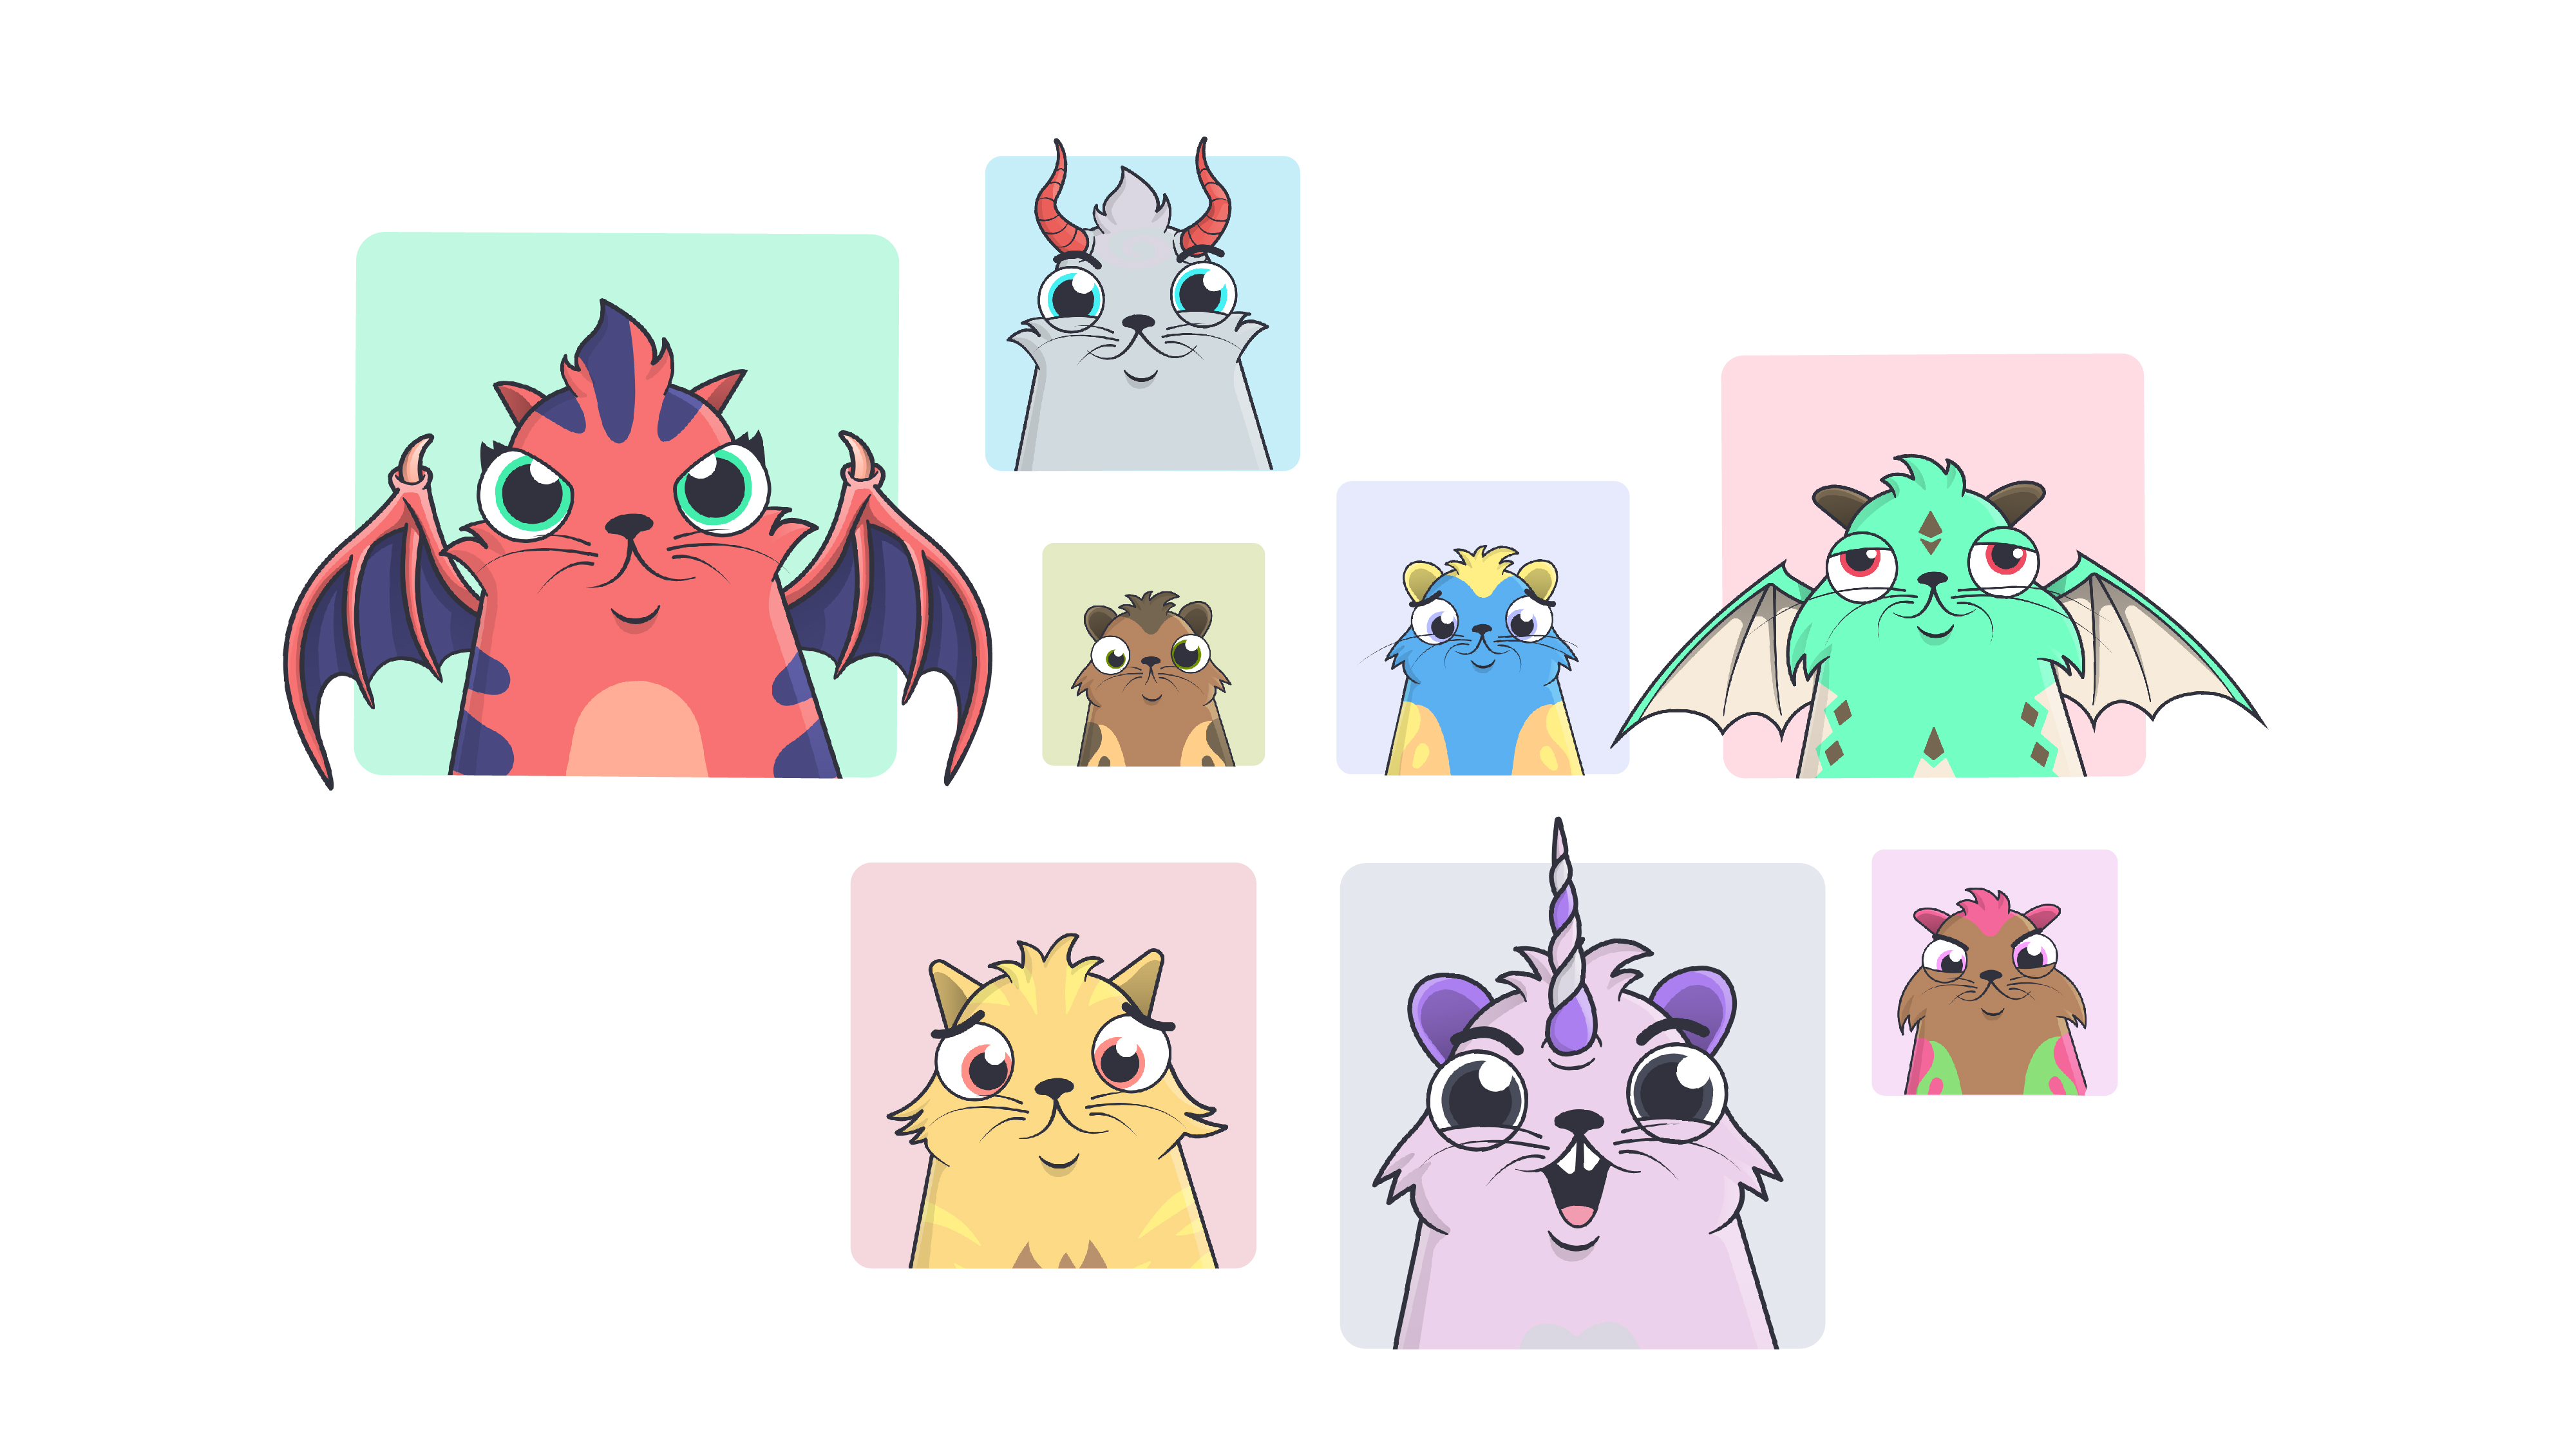
\includegraphics[width=1\textwidth]{press pack_v2-33.jpg}
\caption{\label{fig:Cryptokitties}Bannière Cryptokitties.}
\end{figure}
Une des oeuvres emblématiques des NFT et reconnue comme l'une des  premières œuvres est Cryptokitties. 

Déployé en 2017 par une société Américaine, Cryptokitties est un ensemble de chats - ou plutôt créatures qui ressemblent à des chats - qui peuvent être collectionnés. Nous pouvons voir un exemple de ces créatures dans la figure  \ref{fig:Cryptokitties}. 

Ce sont des NFT qui sont basés sur Ethereum. Ethereum est une blockchain qui est souvent utilisée pour les NFT.

\section{Les opportunités dans l'art} % section 5
\subsection{Transparence} % sous section
Les NFT et la blockchain permettent une certaine transparence dans l'art. 
Le suivi des œuvres d'art est une tâche compliquée, aujourd'hui, seuls certains experts peuvent prouver l'authenticité d'une œuvre. Les papiers utilisés pour cette authentification peuvent être falsifiés ou perdus aisément. 

La blockchain permet un suivi grâce à son certificat distribué. Comme dit précédemment, les données d'une blockchain ne peuvent pas être modifiées ou supprimées ainsi un historique est toujours présent. De plus, le certificat est plus facilement diffusable. Cette mesure permet donc une transparence sur l'origine, la valeur mais aussi le prix d'origine de l'œuvre car les données sont sur la blockchain. 

Ces informations maintenues dans une blockchain permettent également aux musées de faire un meilleur suivi des œuvres d'art, et il y a aussi une possibilité de faire des enquêtes et études sur les transactions dans l'art. \cite{jung_current_2022} 

\subsection{Position des artistes} % sous section
Les artistes voient une nouvelle façon de travailler et d'évoluer. Grâce à la blockchain, les artistes peuvent décider de leurs propres conditions de ventes. Mais elle permet aussi le partage de ces œuvres, effectivement, une œuvre en exposition ne peut être achetée que par une personne alors que sur la blockchain l'œuvre peut être partagée entre plusieurs acheteurs.

Les artistes pouvant choisir leurs positions, nous entrons dans une approche centrée artiste et non plus consommation. Cette approche permet  également aux artistes d'avoir une nouvelle source de rémunération. Précisément, les acheteurs peuvent désormais être à l'autre bout du monde et ne doivent plus se déplacer. Tout cela ouvrant donc de nouvelles possibilités d'achats. \cite{whitaker_art_2019}
Il y a également une réduction des coûts pour les artistes car ils ne doivent donc plus payer les intermédiaires.

\section{Risques associés} % section 6
\subsection{Violation des copyrights} % sous section
Avant d'acheter une NFT, il faut bien vérifier les auteurs et les droits appliqués dessus. En effet, certaines start ups de NFT n'ont pas les autorisations nécessaires pour pouvoir vendre ces NFT et il s'agit là de violation des droits des artistes. 

Nous pouvons prendre le cas de Banksy, une de ses oeuvres a été recréée en NFT mais l'originale a été brûlée. Cette NFT, vendue par "Morons NFT", a donc gagné en valeur car elle devient l'originale. Hors, Morons NFT n'a jamais eu l'autorisation de Banksy de créer cette NFT, elle ne respecte donc pas les copyright. Il faut donc toujours rester attentif avant d'acheter une NFT. \cite{lydiate_crypto_2021}
\subsection{Diversité} % sous section
Tout le monde ne connaît pas la blockchain. Au contraire, c'est une technologie qui peut paraître compliquée et il faut donc les connaissances pour pouvoir l'utiliser. Certaines organisations ont déjà du mal avec la digitalisation de manière générale alors les NFT et la blockchain semblent inconcevables. \cite{abbate_blockchain_2022}

La blockchain demande également de changer la vision de centrer humain à centrer technologie. Le grand public n'a pas forcément accès à la blockchain. Elle peut donc être complexe et seuls les codeurs comprennent celle-ci. Ce n'est donc pas facilement accessible aux publics. 
\subsection{Environnement} % sous section
L'utilisation des NFT de manière générale aurait un impact sur l'environnement. La blockchain et les NFT sont basés principalement sur l'Ethereum qui se base sur un principe de minage. Le minage est le fait de créer un NFT. Hors le minage demande une grande capacité énergétique. Cette consommation énergétique est donc liée à l'environnement. 

L'électricité coûtant le moins cher en Chine, souvent les entrepreneurs vont investir leurs minages là-bas. Hors, l'électricité en Chine est produite encore du charbon, ce qui a un grand impact sur l'environnement. \cite{abdou_prospects_2021} 

De plus, la création de NFT crée des déchets électroniques. En effet, le minage demande une grande capacité de calculs compliqués, il faut donc des puces performantes pour y arriver mais elles arrivent à expiration beaucoup plus rapidement qu'à usage "normal".

Cependant, ce risque pourrait être résolu dans les années à venir grâce des systèmes moins énergivores. 

\subsection{GDPR} % sous section
La question de transparence dans la blockchain peut être à double tranchant. Il est très intéressant de retrouver toutes les informations nécessaires par rapport à l'oeuvre. Cependant, comme dit précédemment, aucune donnée ne peut être supprimée d'une blockchain, il y a donc une trace permanente. 

D'un point de vue GDPR, toute donnée devrait pouvoir être oubliée si l'utilisateur le désire. De ce fait, le règlement général sur la protection des données ne peut pas être respecté. Nous retrouvons donc un souci de confidentialité.
\section{Aspects juridique} % section 7
La définition juridique d'une NFT est compliquée à gérer encore aujourd'hui. Nous ne pouvons pas véritablement considérer une NFT comme une œuvre d'art.  Du fait que les NFT représentent souvent des œuvres d'arts, il nous semblerait logique de les qualifier ainsi. Pourtant du fait de sa technologie, une NFT n'est qu'un processus de tokenisation et donc ne peut être considérée comme une œuvre d'art physique (toile ou tableau par exemple). D'un point de vue fiscal, une œuvre d'art est créée à la main et sans l'aide d'un procédé quel qu'il soit. 

De plus, la génération d'une NFT n'est pas un processus créatif et n'a pas l'empreinte de l'artiste. Les acheteurs ne reçoivent qu'un fichier numérique sur une blockchain et non pas une œuvre sous-jacente. Ils ne sont donc que propriétaires du support de l'œuvre et non pas de l'œuvre en question.  \cite{meghraoui_les_2022}

\section{Avenir} % section 8
Pour l'avenir, les premières questions seront d'un point de vue juridique. Il faudrait effectivement trouver comment définir les NFT afin de pouvoir protéger les vendeurs et les acheteurs de celles-ci. Sans cela, la protection des utilisateurs sera toujours plus compliquée et les fraudes pourraient arriver de plus en plus. 

Le deuxième point serait de trouver une alternative écologique pour le minage de la blockchain. Pour le moment, elle utilise trop d'électricité et des études sont en cours pour trouver des solutions durables tant sur le plan écologique qu'économique. 

La blockchain et les NFT peuvent apporter un bon suivi, pour les musées et les expositions d'arts, de par leurs transparences mais il faudrait que ces institutions s'appliquent d'avantages pour les comprendre. Des études pourraient se faire afin de prévoir si c'est un bon investissement ou non pour celles-ci. 
\section{Conclusion} % section 9
En conclusion, le web 3.0 propose des points positifs et négatifs dans l'art. 
Pour rappel, le web 3.0 serait un web décentralisé et géré par les utilisateurs sans entité unique.

Les NFT (Non fungible Tokens) sont donc des jetons non fongibles, c'est-à-dire des données authentiques et non interchangeables. Elles représentent en général des illustrations numériques. Un des premiers NFT et des plus connus est Cryptokitties. 

La blockchain, elle, est une chaîne de blocs contenant un identifiant unique. Ces technologies sont sur des serveurs partagés par plusieurs utilisateurs. 

Les apports de la blockchain et des NFTs peuvent avoir des points positifs dans l'art. Tel que la transparence, c'est un point qui est intéressant pour prouver l'authenticité d'une œuvre. Les données sur la blockchain ne pouvant pas être modifiées ou supprimées par la suite, il y a un historique et donc un certificat diffusable plus facilement. 

Mais également, la position des artistes, les artistes voient une nouvelle façon de travailler s'ouvrir à eux. Le partage des illustrations est plus simple et ouvert au monde entier. Ainsi, ils touchent un plus grand public, leur offrant une nouvelle source de rémunération. 

Il y a cependant des points négatifs. Nous pouvons retrouver des violations de copyrights, en effet, certaines illustrations et œuvres ne sont pas vendues en toute légalité. C'est-à-dire que les entreprises les vendant n'ont pas les autorisations des artistes. 

Nous retrouvons aussi un problème de "diversité", la blockchain peut être une technologie compliquée d'un point de vue du public. Elle n'est donc pas accessible à tous. 

Pour ce qui est de l'environnement, les NFTs impactent celui-ci pour le moment avec des déchets électroniques dû à une utilisation trop intensive des puces et du fait qu'il faut une grande utilisation d'électricité pour le minage. Actuellement, des solutions sont envisagées et réfléchies afin de régler le problème. 

Et enfin, nous retrouvons des problèmes de protection des données. L'historique de la blockchain est effectivement problématique. Les données ne peuvent être supprimées, hors le règlement général sur la protection des données stipule qu'il y a un droit à l'oubli. Celui-ci n'est donc pas respecté.

Les aspects juridiques des NFT sont encore compliqués à définir. Nous ne pouvons pas définir une NFT comme une œuvre d'art car celle-ci n'est pas créée à la main mais avec l'aide d'un procédé. Il y a donc des débats pour définir juridiquement ce qu'est un NFT afin de protéger les utilisateurs de ceux-ci.

Ces avantages et inconvénients ne sont pas une liste exhaustive et peuvent encore être complétés au jour le jour au vu de l'évolution des NFT et de la blockchain. 

\break
\printbibliography[
heading=bibintoc,
title={Bibliographie}]
\end{document} % fin du corps du texte